
\section{Task A}
For our environment we decided to make a graph structure based upon a set of
"Cells", which has links to its four adjacent neighbors, left, right, up and 
down. By doing so we can make intricate shapes and save memory in doing so. By
using a graph structure we can create complex environments, regardless of size,
with different shapes and connect multiple environments with passageways and
different elements within the environment.

By doing so we also ensure that the agent can easily move from and to cells by
simply going to an adjacent cell, using the links.  Since it is a graph
environment it is also possible to implement graph searching algorithms to find
solutions to different problems.

The environment is very modular because it consists of seperate "cells" which
links to one another.  As shown in figure \ref{fig:env}

\begin{figure}[h] \label{fig:env}	\centering
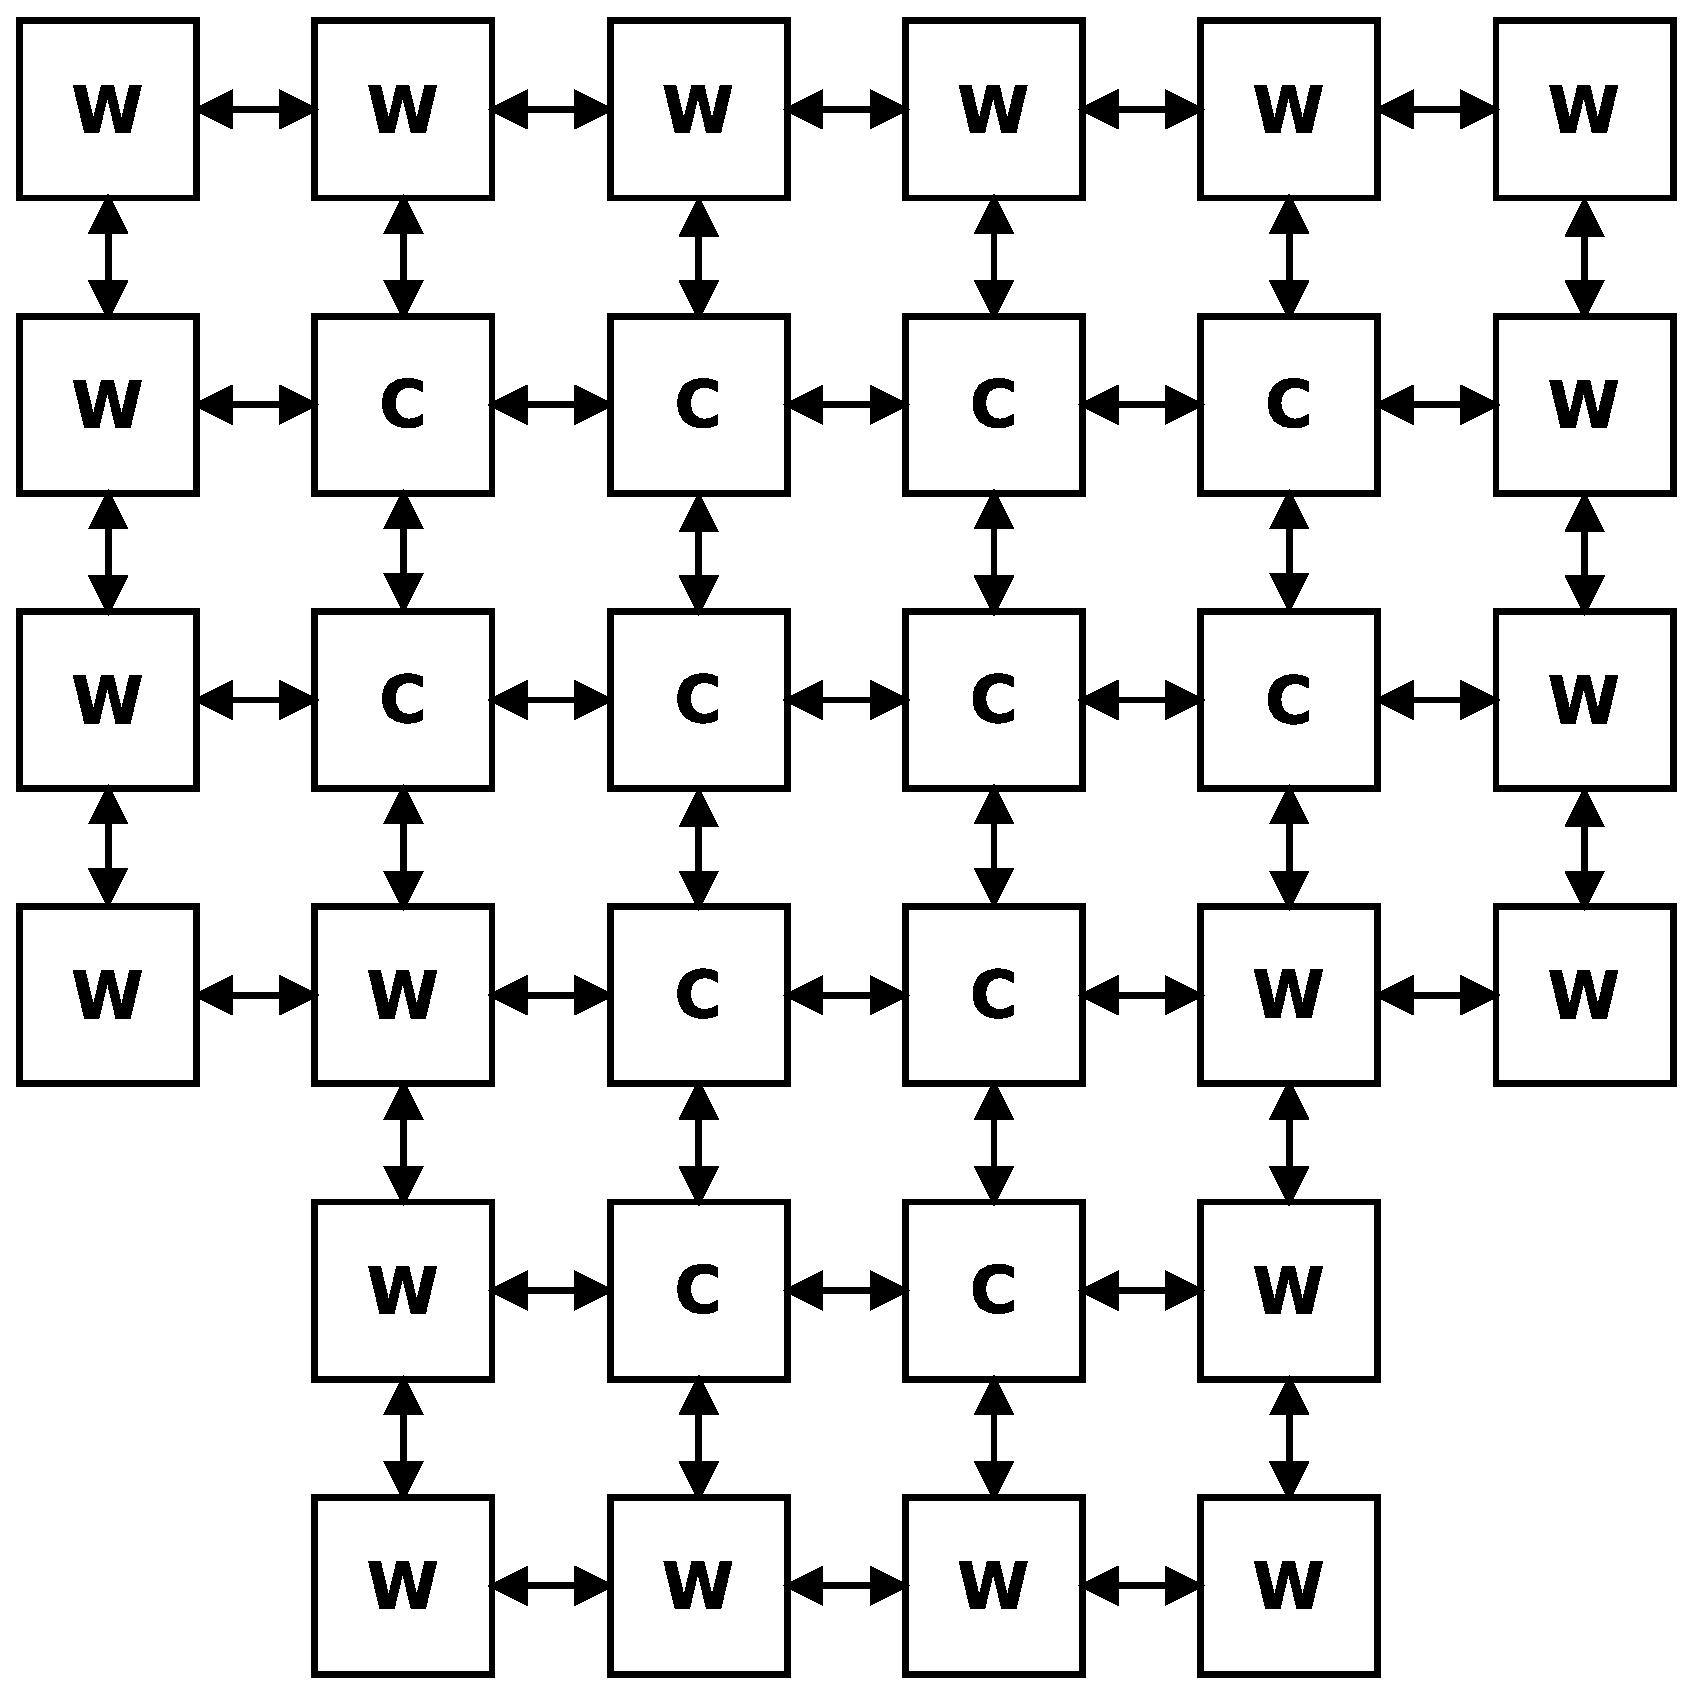
\includegraphics[width=0.6\textwidth]{environment}
\caption{Depiction of an environment}
\end{figure}

\subsection{Cell}
A cell is shown in figure \ref{fig:cell}. A cell is an object that holds
certain information about its current state and links to each of its four
adjacent cells.  The information it holds are:
\begin{description}
\item[key:] 
This integer holds the unique ID of the cell, which is used to search identify 
it during searches. It is specially used during creation of the environment, 
using the createMap() function in "main.cpp";

\item[type:]
Depicts the type of cell by using an integer.  The global ENUM variable sets the
different types as OPEN, WALL and OBSTACLE which is later used in comparisons.

\item[dirty:]
This boolean value states whether or not the current Cell is dirty or not. If it
is true the agent should suck it.

\item[age:]
This holds the information of how many steps it's been since it was last
cleaned.

\item[visited:]
Holds the state of wether the Cell has been visited by the agent. It is not
currently used, but would be to great help in a potential algorithm. For
instance if you need to mark visited cells to avoid getting stuck in a loop .

\item[neighbor:]
This is the four links to the adjacent neighbors; left, right, up and down. The
neighbors can either be set or be NULL if they are the border cell.

The setNeighbors function will set all four neighbors by calling the
setNeighbor(int, Cell*, Cell*) which sets the Cells neighbor as indicated by the
integer(LEFT, RIGHT, DOWN or UP).  Then this function will in return call the
new neighbors setNeighbor(int, Cell*) which creates a link back to the current
Cell.
\end{description}

\begin{figure}[h] \label{fig:cell}	\centering
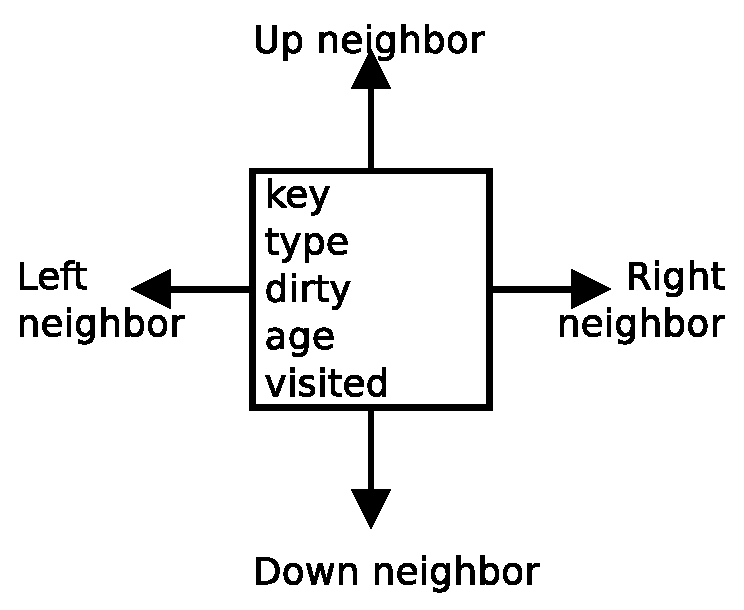
\includegraphics[width=0.5\textwidth]{cell}
\caption{Depiction of a cell and its information}
\end{figure}


\subsection{Environment}

As statet the environment is built up by creating and linking Cells together in
a graph structure. The environment is created by the createMap() function which
reads the graph structure from a file.  The file format is a set of Cells
described by their type and left and right neighbor in a specific order starting
from the far left side.

The file format is [TYPE] [LEFT] [RIGHT]. Where the type is either W for wall, C
for open space and O for an object. LEFT and RIGHT is an integer value
describing the key of the Cell to link to.  This is critical that the keys are
correct and allready created.  The keys are automatically generated during
creation, starting at 1.  Because of this it is important that the cells are
created in correct order so the key exists when linking a new Cell.  If the
RIGHT/LEFT is 0 it will set the neighbor to NULL.

\subsection{Creation}
The Cells are contained in the form of two representations.  The first is the
graph where cells link to each other, and the second is a list which has a
pointer to a Cell and a pointer to the next member of the list, see figure
\ref{fig:list}. The purpose of the list is to enhance the searching speed when 
finding an existing Cell.

Creation of the environment is done by reading the file with the mappings and
creating the new cell without any neighbors. Then it sets the neighbors. After
this it will create the new list-member with a pointer to the Cell-object.

Then this list member will be added to the list before continuing creating the
rest of the cells.

To get a hold of the environment and the list there are created to static
variablels which holds the first element of the list and the first Cell.

\begin{figure}[h] \label{fig:list}	\centering
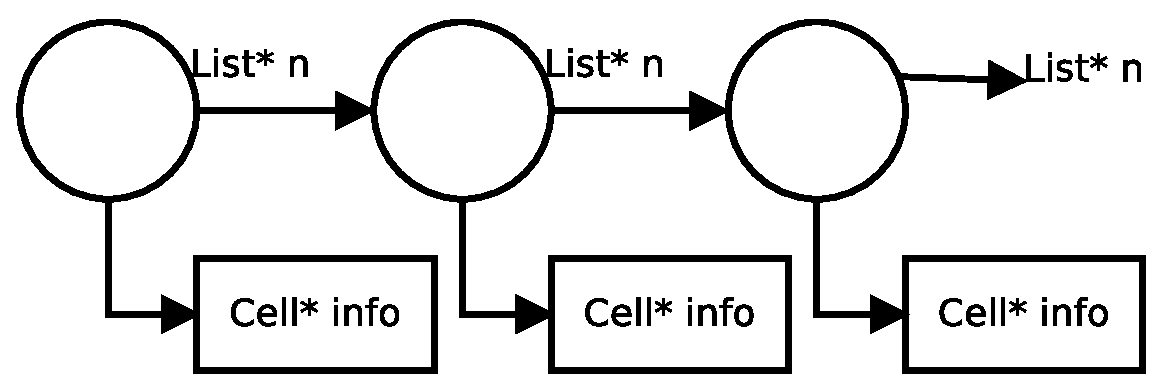
\includegraphics[width=0.75\textwidth]{list}
\caption{Depiction of the list representation of cells}
\end{figure}

